\documentclass[fleqn]{article}
% v3 2013-01-14
% v2 2008-01-17
% v1 2002
\usepackage{brochure}
\def\wLaTeX{L\kern-1.667ex\raisebox{.5ex}{\fontsize{70}{0}\selectfont
    \textsc{a}}\kern-1ex T\kern-1ex\raisebox{-1ex}{E}\kern-.9ex X}
\begin{document}
\noindent\begin{tabular}{
  @{}%	                   flush left margin
  b{.35\columnwidth}%	   logo
  @{\hspace{.03\columnwidth}}%        gap
  >{\huge\centering\color{DarkBlue}}p{.62\columnwidth}%	   headline
  @{}%                     flush right margin
}
  \raisebox{-55pt}{%
    \fontsize{80}{0}\selectfont\color{DarkGreen}\bfseries\wLaTeX}
&
  Sophisticated professional typesetting\\[4pt]\hrule\vspace*{7pt} 
  for business and academic publishing\par\vspace{8pt}\hrule height3pt
  \par\bigskip
  \fontsize{16}{18}\selectfont\itshape
  The ideal solution for your document formatting\linebreak
  and database or {\Large XML} publishing requirements
\end{tabular}

\vfill

\noindent\begin{tabular}{@{}
                         p{.38\columnwidth}%		blurb
		         @{\hspace{.04\columnwidth}}% 	gap
		         p{.58\columnwidth}%		quotes
		         @{}%			implicit margin
}
\sffamily\lite\fontsize{16}{18}\selectfont\raggedright 
The ultimate in portable typesetting: \LaTeX\ runs on \\any computer
and produces timely, accurate output in publication quality on your
desktop printer or business typesetter. 
\par\medskip
\LaTeX\ is completely free, and has been the tried and tested solution
for over 25 years.  
\par\medskip
\LaTeX\ is in use by leading publishers, documentation specialists,
and technical and academic users worldwide.

\small\rightskip=0pt
\subsection*{\sffamily What they say about \LaTeX}
I was getting increasingly exasperated with the limitations presented
by wordprocessing programs when \LaTeX\ came into my life and
allowed me to do all those things I previously could only dream of,
from unusual symbols to complicated layout. I strongly recommend it
to anybody interested in producing a professional-looking document!
\quoted{Petra Hellmuth, Language Specialist}
\par\medskip
I use pdf\LaTeX\ and \MF\ not only because I need them to create my
presentations, lecture notes and papers but also because it's fun!
Entering a math equation in Powerpoint is a pain in the neck: with
pdf\LaTeX\ and \MP\ it is a lot easier because you can change the
style of what is to be displayed. I have a lecture class from which I
generate a lecture presentation \emph{and} lecture notes all from the
same source: I can add text which appears in one or both of the
documents.
\quoted{Marc van Dongen, Computer Scientist}
\par\bigskip
%\vbox to7pc{\hrule\hbox to\hsize{\vrule height7pc\hfill\vrule}\hrule}
\begingroup
  \setlength{\fboxsep}{3pt}\noindent
  \fbox{\vbox to8pc{\hsize=.38\columnwidth
    \advance\hsize by-2\fboxsep\advance\hsize by-2\fboxrule
    \null\vfill\normalsize\centering
    \LaTeX\ is available in Ireland from
    \par\medskip\footnotesize\tabcolsep1mm
    \begin{tabular}{p{.4\hsize}p{.55\hsize}}
      Silmaril Consultants\par
      Bishopstown, Cork\par
      \url+latex@silmaril.ie+\par
      \scalebox{.94}[1]{\url+http://silmaril.ie+}
      &
      UCC Computer Centre\par
      Electronic Publishing Unit\par
      3.19 Kane Building\par
      \scalebox{.94}[1]{\url+http://epu.ucc.ie/latex/+}
    \end{tabular}\par\medskip
    The Irish \TeX\ And \LaTeX\ Interest Community (ITALIC)
    \\has a mailing list which you can join at\\
    \url+http://listserv.heanet.ie/italic-l.html+
    \vfill}}
\endgroup
&\large
% front RH blurb
\lettrine[lines=3]{I}{f} you need to produce a document for
publication you want robust, professional software which won't let you
down~--- whether it's an annual report, a manual for your customers, a
business plan or white paper for your investors, an article for a
journal, a book for a publisher, a newsletter for your club or
society, or a leaflet or brochure for a product, event, or venue.

\begin{itemize}[noitemsep]

\item \LaTeX\ is a document preparation system for producing
  high-quality output, based on Don Knuth's revolutionary
  \TeX\ typesetting program. It's been used by millions since its
  launch in 1985, and has been continuously updated to bring you the
  state of the art in accuracy and flexibility.

\item More powerful than a wordprocessor or desktop publishing system,
  \LaTeX\ has a host of unique features which can dramatically cut
  time and cost for any publishing project, especially for long or
  complex documents.

\item Its secret is programmability: hundreds of prewritten templates
  (packages) to handle almost any formatting task~--- or you can
  define your own with the underlying style language. You only have to
  define a pattern once, and all further occurrences then follow that
  style, giving it unrivalled consistency: the key to
  professional-looking output.

\end{itemize}

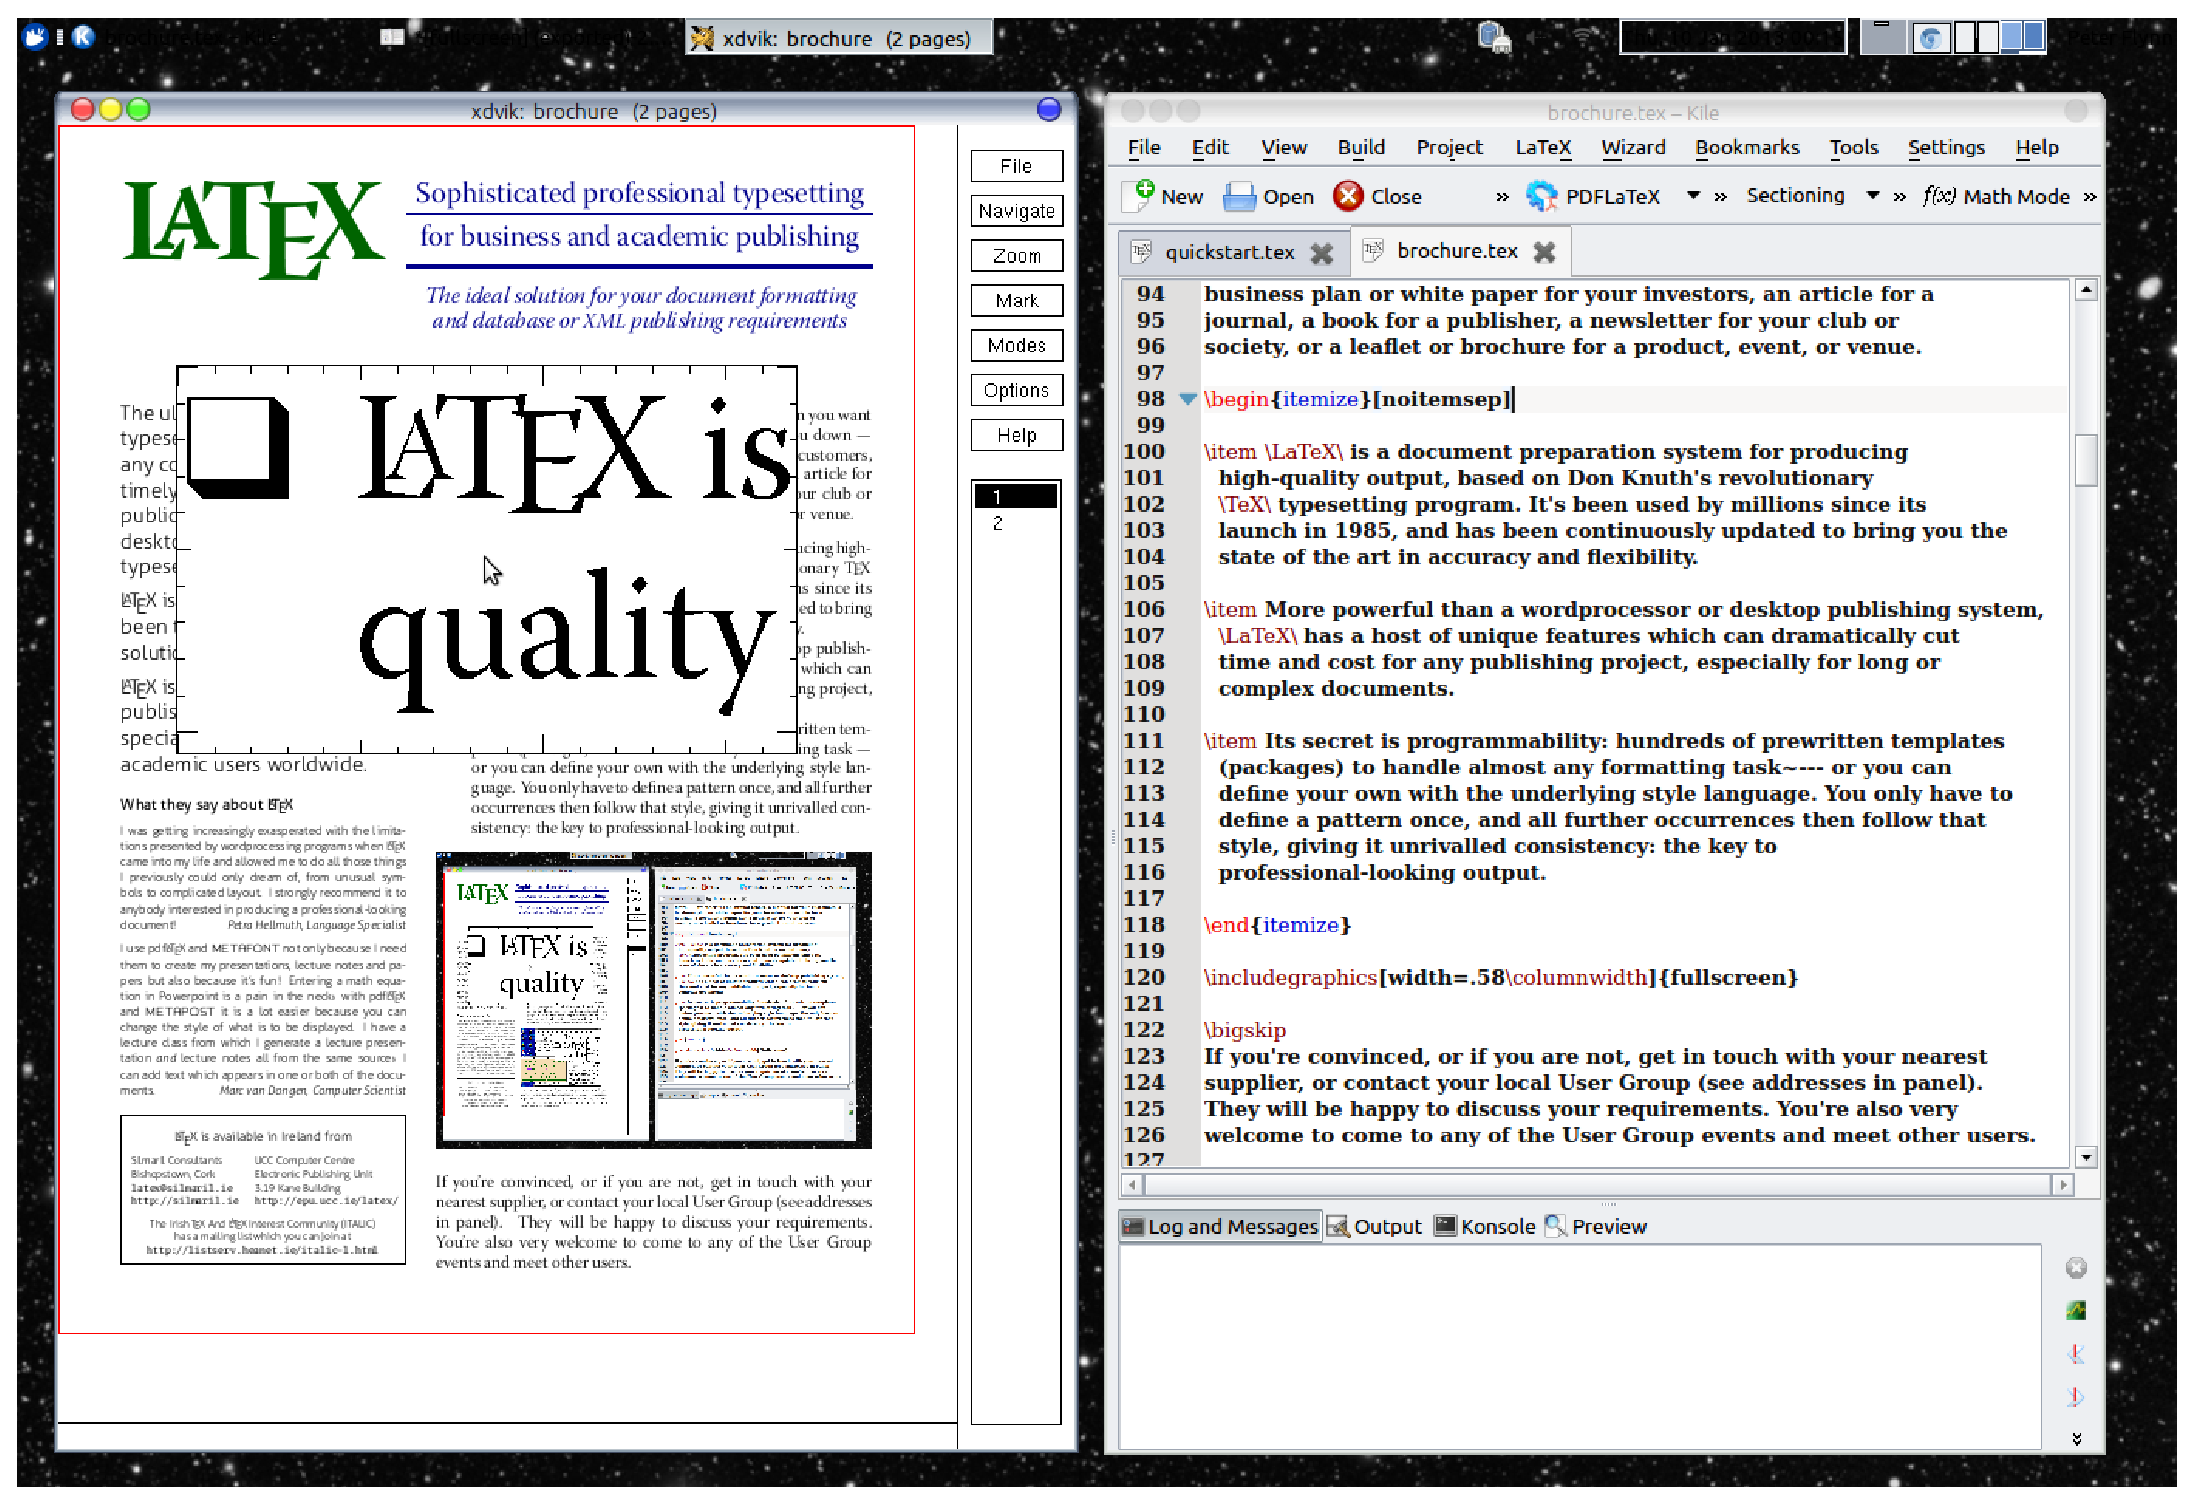
\includegraphics[width=.58\columnwidth]{fullscreen}

\bigskip
If you're convinced, or if you are not, get in touch with your nearest
supplier, or contact your local User Group (see addresses in panel).
They will be happy to discuss your requirements. You're also very
welcome to come to any of the User Group events and meet other users.

\end{tabular}

\clearpage

%%%%%%%%%%%%%%%%%%%%%%%%%%%%%%%%%%%%%%%%%%%%%%%%%%%%%%%%%%%%%%%%%%%%%%%%
%
% P2Inside
%

\noindent\tabcolsep.02\columnwidth
\begin{tabular}{@{}%
    >{\setlength{\leftmargini}{12pt}}p{.32\columnwidth}%
    |%
    >{\setlength{\parindent}{1em}\setlength{\parskip}{2pt}\sffamily}p{.64\columnwidth}%
    @{}%
}
\RaggedRight\null\vspace{-1em}
\subsection{Publishing with \LaTeX}

Could your next report, white paper, article, book, paper, review, or
essay benefit from using \LaTeX? Do you need to be able to exchange
documents with colleagues using other types of computer,
without loss of formatting?

\begin{itemize}[noitemsep]

\item Default styles give you immediate, automatic draft formatting
  for common types of document.

\item Powerful automation features handle cross-references,
  bibliographic citations, tables of contents, indexes, and glossaries
  with ease.

\item Automated formatting of formulae, designed by one of the world's
  leading computer scientists.

\item Industry-standard Acrobat (\textsc{pdf}) and PostScript
  (\textsc{ps}) output.

\item Available in Open Source and commercial versions.

\item Strongly supported via the Internet, with user groups in many
  countries, and by business-level consultants and vendors.

\item Huge range of fonts and languages supported, with floating and
  fixed accents, hyphenation, and language-based typographic
  rules.

\item Journal and book style files available from leading publishers.

\item Available on almost all platforms: \textsc{pda}s, smartphones,
  and tablets; laptops and desktops; minicomputers, mainframes, and
  supercomputers.

\item Completely portable between systems~--- document files are all
  plain Unicode and can be edited and processed on any supported
  platform.

\end{itemize}

\subsection{Mathematics}
Automated mathematical formatting uses a symbolic notation, regardless
of complexity. Spacing and sizing is done to
mathematicians' standards, so this:
\par\medskip
\begingroup\fontsize{7.25}{8}\selectfont
\verb`E(n_{g+1}'|n_i',n_i'';\,1\le i\le g)=(N'-`\linebreak
\verb`N_g')\left[1-\left\{\left(1-\frac{c}`\linebreak
\verb`{cN'+N''}\right)^{n_g'd}\left(1-\frac{c}`\linebreak
\verb`{cN''+N'}\right)^{n_g''d}\right\}\right]`
\par\endgroup\smallskip
results in the equation below. Graphical \LaTeX-based systems
such as \LyX\ and \textit{Scientific Word} have built-in equation
editors for constructing expressions with the mouse and menus.
&
\null\vspace{-2.5em}
\subsection{\sffamily Typefaces}

\noindent Whether you're using Windows or Unix (including Apple Mac
OS\thinspace X and GNU/Linux systems), standard \LaTeX\ works with any
Type~1 outline (PostScript) or Type~3 bitmap (\MF). Using the
\XeLaTeX\ processor (included on the DVD),
you can also use all your TrueType and OpenType fonts. This gives you
access to tens of thousands of typefaces, both free and commercial.

The standard Adobe `35' core PostScript fonts (Times, Palatino,
Century Schoolbook, Helvetica, Zapf Calligraphic. etc) are provided by
default; with the mathematics fonts of Computer Modern,
Euler, Concrete, and Times; and a range of decorative and specialist
typefaces for technical, linguistic, and literary typesetting.

\bigskip\noindent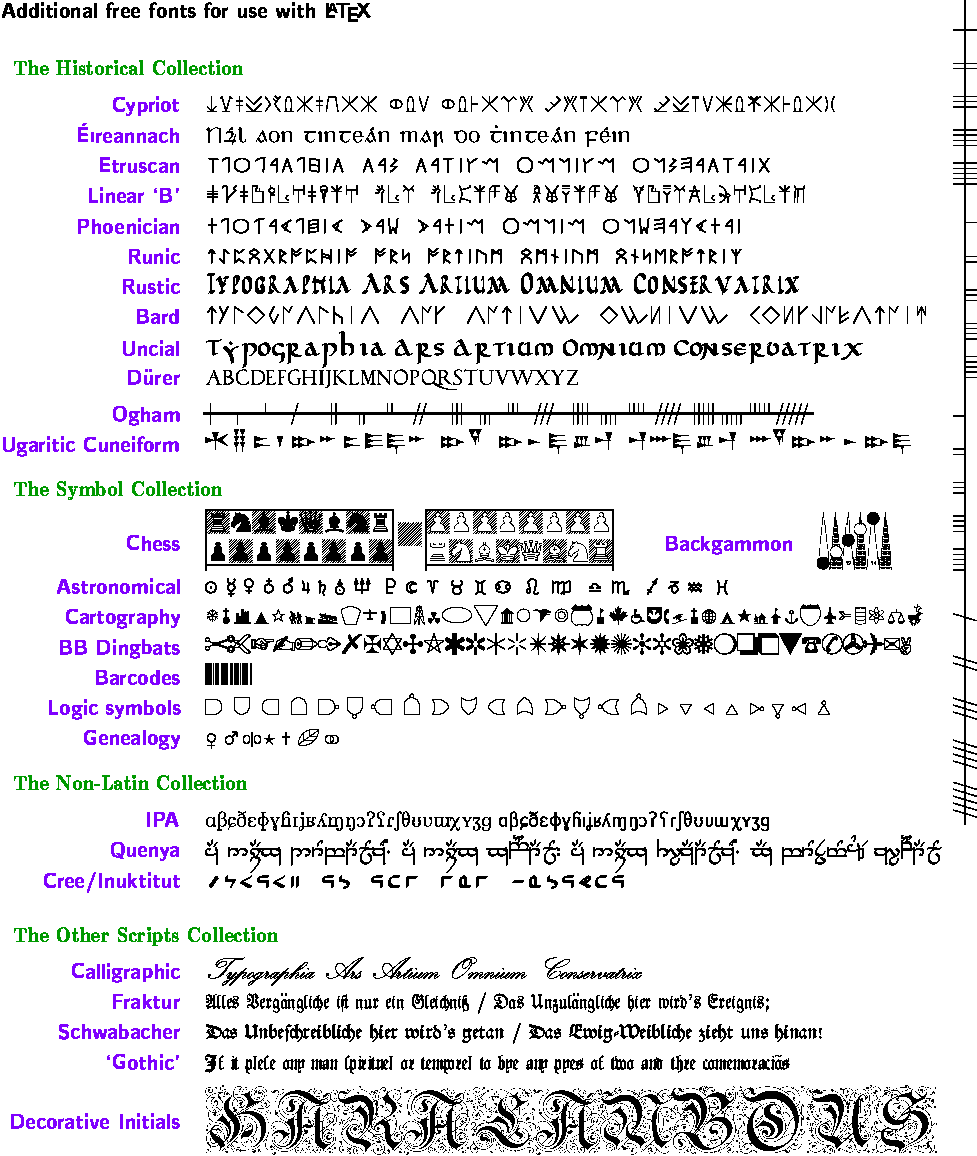
\includegraphics[width=.6\columnwidth]{sample-crop}
\par\bigskip

Non-Latin types include Japanese, Chinese, Devanagari, Urdu, Thai,
Vietnamese, Coptic, Cyrillic, Greek, and many other languages and
alphabets, including mixed bi-directional Arabic and Hebrew. Extensive
user group coverage world-wide provides native-language support for
non-Latin typesetting.

The fontmaking programs \MF\ and \MP\ come with all
\TeX\ systems for designing and implementing your own
typefaces or special symbols.

The calculations of the underlying \TeX\ formatting engine are very
precise: it works internally in microunits smaller than the wavelength
of visible light ($\approx$53.6\AA), resulting in great accuracy in
positioning. \LaTeX\ can use any mixture of Anglo-American, Didot, or
Adobe points, or metric or imperial units.
\\\cline{2-2}
\end{tabular}
\par\vfill
\begingroup
\setcounter{section}{10}
\setcounter{equation}{56}
\renewcommand{\theequation}{\thesection.\arabic{equation}}
\begin{equation}
E(n_{g+1}'|n_i',n_i'';\, 1\le i\le g)=(N'-
N_g')\left[1-\left\{\left(1-\frac{c}
{cN'+N''}\right)^{n_g'd}\left(1-\frac{c}
{cN''+N'}\right)^{n_g''d}\right\}\right]
\end{equation}
\footnotesize 
After Rapoport (in Bartholomew, D.J. \textit{Stochastic Models for
Social Processes}, 2nd.\ ed., John Wiley \& Sons, 1973,
p.\thinspace368.)\par\endgroup
\vfill
\clearpage

\begin{multicols}{3}\setlength{\parindent}{1em}
\subsection{Tables} 

\LaTeX's tables and figures follow the standard publishers' practice
of `floating', so if there is no room on the current page, they
automatically float to the next. Automated crossreferencing means that
tables and figures can be moved around the document and will always
renumber themselves and all their references.
\par\bigskip 

\begingroup 
\setlength{\bigstrutjot}{\jot}
\def\vstrut{\vrule depth.5pc width0pt}
\renewcommand{\multirowsetup}{\centering} \setlength{\tabcolsep}{1pt}
\setlength{\arrayrulewidth}{.1pt} \scriptsize\normalfont\noindent
\textsc{Table 6.2: cases for which the Quantile and Kemsley's methods
  were impossible, classified by the size of
  $\sigma$}\par\smallskip\noindent
\begin{tabular}{%
    @{\vrule height1pc depth.5pc width0pt}|
    c|
    >{\columncolor{SpringGreen}\quad}c<{\quad}|
    >{\columncolor{Lavender}\enspace}c<{\enspace}|
    >{\columncolor{SpringGreen}\quad}c<{\quad}|
    >{\columncolor{Lavender}\enspace}c<{\enspace}|
    c|@{}}\hline
  \multirow2{2pc}[-1em]{$\sigma$}
  &
  \multicolumn2{p{3pc}|}{\centering Method of\par quantiles\vstrut}
  &
  \multicolumn2{p{3pc}|}{\centering Kemsley's\par method\vstrut}
  &
  \multirow2{3pc}[-.5em]{Total no.\ of samples available}
  \\\cline{2-5}
  &5\%&10\%&5\%&10\%&\\\hline
  0.2--0.4&2&1&1&4&20\\[-9pt]
  0.5--0.7&---&---&---&4&22\\[-9pt]
  0.8--1.0&---&1&2&15&23\\\hline
  \rowcolor{LightGoldenrod}\ All samples\kern2ex&2&2&4&23&65\\\hline
\end{tabular}
\par\flushright{\tiny After Aitchison, J. and J.A.C. Brown,\\
\textit{The Lognormal Distribution}, CUP, 1976, p.\thinspace
62.\par}
\endgroup

\medskip
There are powerful tabular controls for both simple and complex
designs, with fixed or auto-adjusting spacing which can be very
precisely aligned to provide better visual appeal.  Formal tables and
Figures are automatically numbered, and can be captioned, labelled,
crossreferenced, and included in a List of Tables and List of Figures.

Complex tabular matter can span pages and can be printed landscape
while retaining the portrait orientation of the caption and
pagenumber.  Simple tabular matter can appear anywhere, without being
a formal numbered table.

\subsection{Crossreferences}

The crossreferencing features let you name anything you want to refer
to (table, figure, section, chapter, page, item, etc), and then use
that name anywhere in the document.
This lets each crossreference automatically update its location so
that no matter how much you edit the text, the references remain
correct. The same method is used for automated indexing, glossary,
table of contents, list of figures, list of tables, and bibliographic
references.

The \BibTeX\ bibliographic database lets you store references
separately from documents, and the \BibLaTeX\ system extracts and
automatically formats them to any of the standard styles, including
numeric, in-text, footnotes, or endnotes.

\subsection{Figures and illustrations}

Figures can contain textual or graphical illustrations. Pictures can
be included with scaling, rotation, and clipping, using industry
standard PDF or EPS vector formats for diagrams, or PNG or JPG bitmaps
for pictures.
\par\medskip\noindent
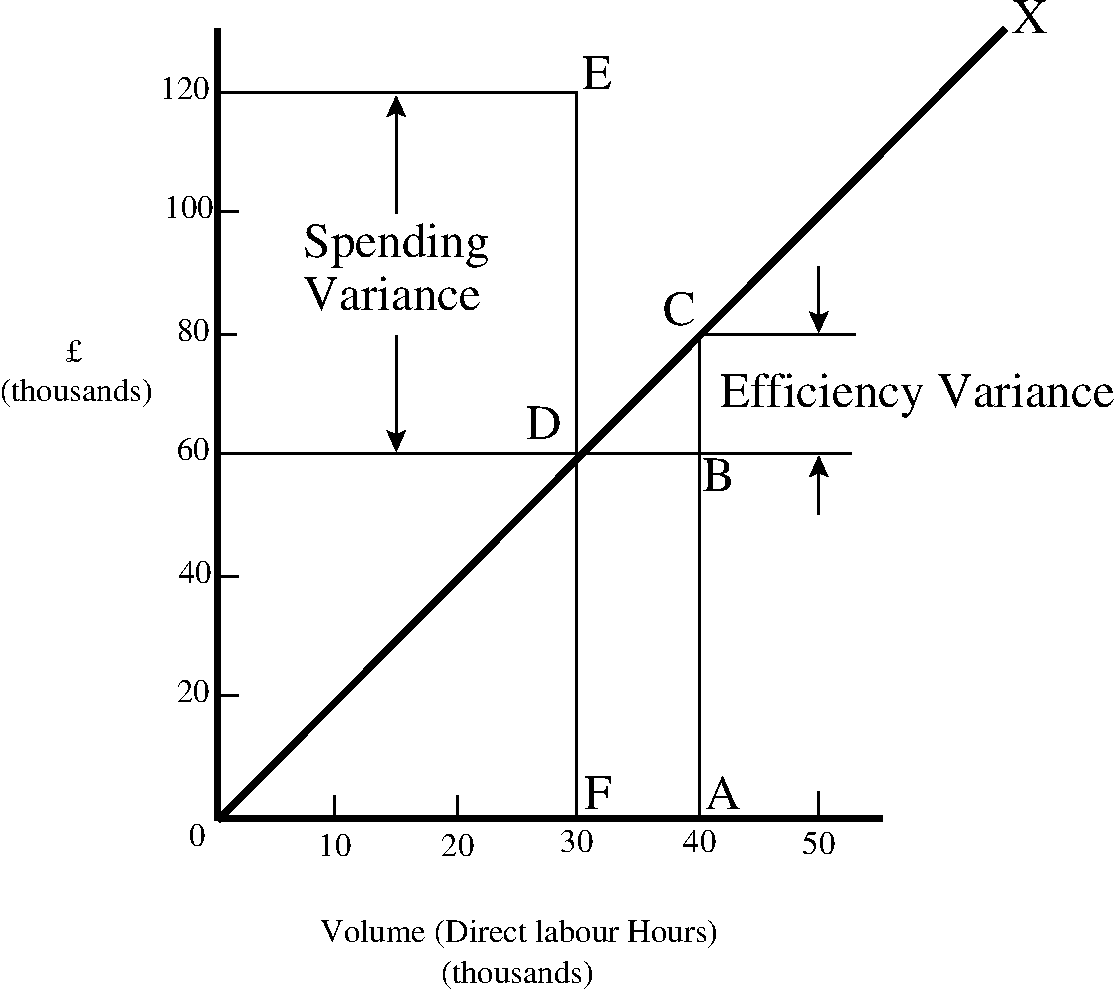
\includegraphics[width=\columnwidth]{diagram-crop}
\par\vspace{-6pt}\begingroup\flushright{\tiny After R.J. Bull,
\textit{Accounting in Business},\\Butterworths, 2nd.\ ed., 1972,
p.\thinspace 191.\par}\endgroup\medskip

\LaTeX\ also has its own CAD-like vector language for simple diagrams,
and there are packages for typesetting music, electronic circuits,
flowcharts, and other graphical notations.

\end{multicols}

\hrule

\begin{multicols}{2}

\begin{multicols}{2}\parskip0pt\parindent0pt
\sffamily\lite\fontsize89\selectfont

\includegraphics[width=\columnwidth]{typo-degraded}
\par{\flushright\tiny
Illustration from collection of Don Knuth (artist
unknown)\par}
\columnbreak
I find \LaTeX\ a powerful instrument for generating elaborate
typographic layouts quickly and reliably. They are available for
revision for years afterwards, without worries about software versions
or compatibility. \LaTeX\ is demanding in its requirements but it
relieves me of any concern about the finished project.\par
\quoted{S\'eamus \'O Dire\'ain, Lexicographer}
\end{multicols}

\renewcommand{\refname}{Documentation}
\nocite{*}
\begin{Sbox}\begin{minipage}{.9\columnwidth}
\scriptsize
\makeatletter\let\@apabi\bibitem\def\bibitem{\vspace*{-.5\baselineskip}\@apabi}%
\bibliography{brochure}
\bibliographystyle{apacite}
\parskip0pt\parindent1em
The book by Lamport is the user manual for \LaTeX: make sure you get
the second edition for \LaTeXe. The \textit{Companion} is more
advanced, but useful if you want to implement your own customised
document designs. Knuth's original \textit{\TeX book} is of interest
mainly to computer scientists and typographic programmers who need to
know the finest detail.

There are dozens of other books, ranging from the online
introductions, \textit{Formatting Information} and \textit{The (not
so) short introduction to \LaTeXe}, to the professional
mathematician's \textit{The Joy of \TeX} and the typographer's
\textit{Digital Typography}.

\end{minipage}\end{Sbox}
\fboxsep1em\noindent\shadowbox{\TheSbox}

\columnbreak
\fontsize{11}{13}\selectfont
\subsection{Persistence and reliability}

\LaTeX\ was designed to be independent of any particular manufacturer,
make, or model of computer or printer. Unlike some wordprocessor
manufacturers' proprietary file formats, \LaTeX\ uses plaintext
(\textsc{ascii} or Unicode) files which can be created and updated
with any editor anywhere, and moved between different systems without
danger of information loss or corruption.

The system has been carefully designed so that documents written years
ago can still be typeset. Because the file format is stable, your
investment in intellectual property cannot be damaged by vendors'
arbitrary or planned obsolescence, or by changes in versions or
formats.

\bigskip\hrule\medskip
\sffamily\lite\small\parindent0pt\parskip1em minus.75em
\LaTeX\ material originally produced for paper printing, no matter how
long ago, can quickly and easily be made available for today's Web
access. I have just recently had to provide a journal from 1987--1996
in a format available for the Web.  The opening page was converted
into HTML for quick scanning on the Web, while the complete articles,
with all typesetting and font features (including Hebrew, phonetics,
and Greek), were available for viewing in PDF just by re-running the
\LaTeX\ files.

The biggest advantage in publishing production is that similar
coding of files means anyone can do any journal~--- there is no
need to learn new sets of commands for style variations.
Changes in platforms have no effect on production as \LaTeX\ is
available for all main operating systems.

It is possible to separate the writing tasks (creation of text) from
the design/layout issues (spacing, fonts, etc), which allows the
author simply to identify types of elements (heading levels,
foot/endnotes, citations, etc) without getting bogged down trying to
remember the text shape and font selections for each element.\hfill
\textit{Christina Thiele}, CCS Publishing

\end{multicols}
\clearpage

% BACK PAGE

% Column 1 is the decorative initial I on its own
% Column 2 is the biblical text
% Column 3 is the caption
\noindent
\begin{tabular}{@{\hspace{2mm}}%			explicit margin
		>{\deco}b{.2\columnwidth}%	initial I
		@{}%			no space
		>{\frak}b{.45\columnwidth}%	illustration (Gutenberg)
		@{\hspace{.02\columnwidth}}% 	gap
		>{\rubric}b{.32\columnwidth}%	captioning
		@{}%			explicit no margin
}
  \raisebox{1.2cm}{I}
&
  N principio erat verb\~u: \et\ verb\~u erat apud de\~u: et
  de\raisebox{3pt}{\LARGE9} erat verb\~u. Hoc erat in principio apud
  de\~u. O\~mia p i\~pm facta sunt: \et\ sine i\~po factum est
  nichil\rlap. Quod fact\~u est in i\~po vita erat: \et\ vita erat lux
  homin\~u: et lux in tenebri\char'215\ lu\rlap- cet$\cdot$
  \et\ tenebre e\~a n\~o com\~phender\~ut. Fu\rlap-
&
  Typographic reconstruction of Gutenberg's 42--line bible of
  1452--55, using modern Fraktur and decorative initial designed in
  \MF\ by Yannis Haralambous.
  \par
  The ability to control special characters like the insular
  (Tironian) ampersand ({\frakfamily\et}) and unusual features like
  hanging punctuation makes \LaTeX\ particularly well suited for
  typesetting critical and teaching editions. 
  \par\itshape 
  (Beginning of St.\ John's Gospel.)
\end{tabular}

\columnsep2em
\begin{multicols}{2}\setlength{\leftmargini}{14pt}

\subsection{Where to get \LaTeX}

\begin{itemize}[noitemsep]

\item The \TeX\ Users Group (TUG) distributes a free copy of the
  \TeX\ Collection DVD to all members annually, with complete
  installations for all major platforms and a copy of the entire CTAN
  archive. 

  Many local and national user groups also participate: check with
  your nearest group (see TUG Web site for addresses).

\item You can buy a copy with business support from any of the vendors
  listed below.

\item All the public-domain and open-source implementations are freely
  available for download from CTAN (below), including the DVD ISO image
  of the \TeX\ Collection.

\end{itemize}

\subsubsection{The \TeX\ Users Group (TUG)}

TUG membership is \$85 a year (individual), \$55 (students, new
graduates, seniors, and citizens of countries with modest economies),
\$100 (non-voting, eg libraries), or \$500 (institutional, up to eight
named memberships).  See \url+http://www.tug.org/forms+ for details of
`early-bird' rates and other charges. Membership includes the
triannual journal \textit{TUGboat} and discounts on conference fees:

\medskip\begingroup\footnotesize\centering\tabcolsep1.2em
\begin{tabular}{@{}lll@{}}
&\scshape tug&\scshape Euro\TeX/Con\TeX t and others\\[3pt]
  2013&Tokyo, Japan&[tba]\\
  2012&Boston, MA&Breskens, Netherlands\\
  2011&Kerala, India&Bassenge, Belgium \& Bachotek, Poland\\
  2010&San Francisco, CA&Brejlov, Czech Republic\\
  2009&South Bend, IN&Pisa, Italy\\
  2008&Cork, Ireland&Bohinj, Slovenia \& Pisa, Italy\\
\end{tabular}
\endgroup

\subsubsection*{CTAN~--- the Comprehensive \TeX\ Archive Network}

CTAN is an Internet archive of all free \TeX\ and \LaTeX\ software,
packages, and documentation. There are searchable indexes and
catalogues at \url+http://www.ctan.org+, \url+http://www.tex.ac.uk/+,
and \url+http://www.dante.de+~.

\subsubsection*{Online and other support}

Network-based support is freely available on the \url{comp.text.tex}
Usenet newsgroup, the \url{latexusersgroup@gmail.com} mailing list and
the \url{tex.stackexchange.com} web forum.  There are many others,
including the \TeX\ FAQ, listed at \url{www.tug.org/interest.html}~.

\subsubsection*{Vendors with business support}

\begingroup\scriptsize\setlength{\tabcolsep}{3pt}\noindent
\begin{tabular}{@{}l>{\itshape}ll>{\ttfamily}l@{}}
  Andrew Trevorrow&Oz\TeX&Mac&http://www.trevorrow.com/oztex/\\
  MacKichan Software&Scientific Word&Win&http://www.mackichan.com\\
  MicroPress, Inc&Visual \TeX&Win&http://www.micropress-inc.com\\
  PC\TeX, Inc&PC\TeX&Win&http://www.pctex.com\\
  Tom Kiffe&CMac\TeX&Mac&http://www.kiffe.com\\
  True\TeX, Inc&True\TeX&Win&http://truetex.com\\
\end{tabular}\endgroup

\columnbreak
\fontsize{11}{13}\selectfont\sffamily

\subsection{\sffamily Technical Requirements}
\subsubsection{\sffamily Operating systems}
\LaTeX\ runs on all current computing platforms. The most common
implementations are:

\begin{center}\small\tabcolsep4pt
\begin{tabular}{|>{\raggedright\vrule height1.5em width0pt}m{3cm}
                |>{\vrule height1.5em width0pt}m{5cm}|}
\hline
  \textbf{System}&\textbf{Implementation}\\\hline
  Microsoft Windows&\textit{Free}: \textbf{\TeX\ Live}, Pro\TeX t
  (Mik\TeX)\par
  \textit{Commercial}: see vendor list\\
  Unix and GNU/Linux&\textit{Free}: \textbf{\TeX\ Live}\\
  Apple Macintosh OS\thinspace X&\textit{Free}: \textbf{Mac\TeX}
  (\TeX\ Live)\par
  \textit{Shareware}: OZ\TeX, CMac\TeX\\
  Android&\TeX\ for Android in the Google Play store\par
  \TeX\ Live for Android at Google Code\\
  All others&\itshape Contact the \TeX\ Users Group\\[3pt]\hline
\end{tabular}
\end{center}

\subsubsection*{\sffamily Hardware}
\begin{itemize}[noitemsep]
\item \LaTeX\ will run even on old machines, but a 500MHz processor or
  above is recommended.
\item You should have at least 512Mb of memory, more if you aim to do
  very complex work or use very long documents.
\item You need about 500Mb of hard disk space depending on the options
  you choose (minimal install is about 250Mb; full is about 1.2Gb).
\item The finer your screen and printer resolution, the better quality
  you will be able to see and print. A fast inkjet printer or a laser
  printer is recommended if you need printed output.
\end{itemize}
\subsubsection*{\sffamily Software for editing and reading documents}
\begin{itemize}[noitemsep]

\item You need a good text editor for creating and maintaining
  documents: there is a selection included on the \TeX\ Collection
  DVD.

\item You also need a PDF reader to view your typeset output (included
  on the \TeX\ Collection DVD), eg
  \textit{GhostScript}/\textit{GSview}, \textit{Okular}, Adobe
  \textit{Acrobat Reader}, etc.

\item You may need a graphics editor (eg \textit{GIMP}) if you want to
  create or modify images (see \textit{Figures}); and a vector editor (eg
  \textit{InkScape}) if you use diagrams.

%\item There is a wide range of other utilities available from the 
%Comprehensive \TeX\ Archive Network.

\end{itemize} 

\end{multicols}
\vfill
\noindent
\begingroup\fontsize56\selectfont \TeX, \LaTeX, and \MF\ are trademarks
  of the American Mathematical Society. PostScript, PDF, and Acrobat
  are trademarks of Adobe Corporation. Macintosh and TrueType are
  trademarks of Apple Corporation. Windows, Word, and OpenType are
  trademarks of Microsoft Corporation. Unix is a trademark of Bell
  Laboratories. Unicode is a trademark of Unicode, Inc. Copyright
  \copyright\ 2001--\number\year\ by Silmaril Consultants and
  distributed under the terms of the \LaTeX\ Project Public License
  (\url{http://www.latex-project.org/lppl/}). 
\par\endgroup

\end{document}
